\documentclass[11pt,leqno,oneside]{amsart}
\usepackage[margin=1in]{geometry}

\usepackage{../notes}
\usepackage{xfrac}
\usepackage{enumitem}
\usepackage{tikz-cd}
\usetikzlibrary{cd}
\usepackage{hyperref}
\usepackage{mathtools}
\mathtoolsset{showonlyrefs}

\usepackage{datetime}
% an environment specifically for my dates, although it doesn't actually depend on datetime:
\newenvironment{dateenv}{
  \vspace{1em}
}{
  \vspace{1em}
}
% my date command, for convenient date adding
\newcommand{\mydate}[4]{
  \newdate{#1}{#2}{#3}{#4}
  % #1 is a unique string, #2 is day, #3 month, #4 year
  \begin{dateenv}
    \hfill\displaydate{#1}
  \end{dateenv}
}

\numberwithin{thm}{section}
\setlength\parindent{0pt}

\everymath{\displaystyle}

\newcommand{\of}{\circ}
\newcommand{\minus}{\smallsetminus}
\renewcommand{\setminus}{\smallsetminus}
\renewcommand{\amalg}{\sqcup}
\newcommand{\homotopic}{\simeq}
\renewcommand{\epsilon}{\varepsilon}
\renewcommand{\d}{\partial}
\newcommand{\fund}{\pi_1}
\newcommand{\transverse}{\pitchfork}
\newcommand{\into}{\hookrightarrow}
\newcommand{\onto}{\twoheadrightarrow}
\newcommand{\x}{\times}
\newcommand{\Map}{\text{Map}}
\newcommand{\id}{\text{id}}
\renewcommand{\bar}{\widebar}
\newcommand{\de}{\emph}

%%%%%%%%%%%%%% BEGIN CONTENT: %%%%%%%%%%%%%%

\title[Algebraic Topology]{Algebraic Topology MATH 7800}
\author{Chris Lloyd, Matthew Lancellotti}
\date{}
\begin{document}
\maketitle \newpage

\mydate{d1}{18}{1}{2017}

\section{Introduction}

Topology is floppy. Given just a topological space one has an infinite
degree of freedom. This makes even simple questions hard to answer, in
particular given manifolds \(M\) and \(N\) with different dimensions
\(m\) and \(n\) respectively, one may ask if they are
homeomorphic. Intuitively one would think that should not be
possible. However there do exist space filling curves, i.e,
\[I \twoheadrightarrow I \times I\]
where as always \(I=[0,1]\).

We will develop the tools to prove manifolds of different dimensions can
certainly never be homeomorphic. Another surface result assures there exists no continuous
retraction \(D^2 \to \d D\), which then immediately yields the
Brouwer Fixed Pointed Theorem (every map \(D^2 \to D^2\) admits a
fixed point).

In this course there will be two basic branches under consideration:
homotopy theory and homology. Basically, homotopy concerns itself with
continuous deformations between maps. While homology studies subspaces
(known as ``cycles'') and gap filling.

\section{Reference}

\begin{defn}
  $D^n$ denotes the $n$-dimensional closed unit disk.
\end{defn}

\section{Homotopy}

We now define homotopies in the space of maps between manifolds \(M\)
and \(N\) denoted
\[\Map(M,N)=\{f \colon M \to N \mid \text{$f$ is continuous}\}.\]

In this course, we follow the convention that maps are continuous
functions unless otherwise stated!

\begin{defn}
  A \emph{homotopy} from \(f \colon M \to N\) to \(g \colon M \to N\)
  is a map \(h\) such that \(h_0=f\) and \(h_1=g\). We say \(f\) and
  \(g\) are \emph{homotopic} if a homotopy between them exists.

  Often we write \(h_t(m)\) for \(h(m,t)\).
\end{defn}

When working with homotopies one often thinks of having the start and
end map already fixed. For maps to be homotopic they must be in the
same path component.

\begin{prop}
  Homotopy is an equivalence relation.
\end{prop}

We denote the homotopy equivalence class of \(f\) by \([f]\).

\begin{defn}
  A \emph{path} in a topological space $X$ is a map
  \[f \colon I \to X.\]
\end{defn}

By convention in this course, we always consider paths up to homotopy,
however we will make a restriction and only consider homotopies that
fix end points \((I,\{0,1\})\). Otherwise every path would collapse to
a point up to homotopy. This is called \emph{relative homotopy}. When
there are no restrictions placed one is working with \emph{free
  homotopy}.

Imagine two paths in \(\R \setminus (0,0)\) which agree on end points,
however each path is on opposite sides of the origin. It is clear that
there exists no end point fixing homotopy between the two paths.

\begin{defn}
  If one has two paths \(f,g\) with \(f(1)=g(0)\) we may define a new
  path
  \[f * g =
    \begin{cases}
      f(2t), & t \in [0,\frac{1}{2})\\
      g(2t - 1), & t \in [\frac{1}{2},1].
    \end{cases}
  \]

  This is called the \emph{concatenation} or \emph{path composition}
  of $f$ and $g$.

  This operation is well defined on homotopy classes, that is if
  \([f]=[f']\) and \([g]=[g']\) then \([f * g] = [f' * g']\). This
  operation may be generalized to \(*_{k}\) where \(k \in (0,1)\),
  simply replace \(\frac{1}{2}\) with \(k\). In this notation
  \(f * g = f *_{\frac{1}{2}} g\). This operation is associative.
\end{defn}

Given a topological space \(X\) with points \(P\), for any two points
\(x,y \in P\) we have a set of homotopy classes with end points \(x\)
and \(y\). These may be thought of as morphisms and the points as
objects in a category. We call this category the Fundamental Groupoid.

\mydate{d2}{20}{1}{2017}

\begin{defn}
  A \de{category} is a directed graph.  Each vertex is called an
  \de{object} and each directed edge is called a \de{morphism}.
\end{defn}
\begin{defn}
  In the category of \de{finite sets}, denoted $\text{FSet}$, the
  objects are the finite sets, each morphism from $A$ to $B$ is a
  function from $A$ to $B$.
\end{defn}
\begin{defn}
  For any field $K$, the category of \de{$K$-vector spaces}, denoted
  $\text{Vect}_K$, has objects that are $K$-vector spaces and
  morphisms that are $K$-linear maps.
\end{defn}
\begin{defn}
  A \de{groupoid} is a category where every morphism has an inverse.

  That is, if $a: x \to x'$, then there exists $a^{-1}:x' to x$
  s.t. $aa^{-1} = \id_{x'}$ and $a^{-1}a = \id_{x}$.

  The elements of the groupoid are the morphisms.  The operation is
  composition.  Not every pair of morphisms can necessarily be composed!
\end{defn}
\begin{prop}
  Every morphism in a groupoid is an isomorphism (by definition).
\end{prop}
\begin{defn}
  A \de{group} is a groupoid with one object.
\end{defn}
\begin{prop}
  If $A$ is an object in a groupoid, then $\Hom(A, A)$ is a group.
\end{prop}

note We see that a groupoid is the same definition of a group, but we
use a *partial* binary operation instead of a binary operation.

\begin{defn}
  The \de{fundamental groupoid} of $X$, denoted $\Pi_1 X$, is the
  category where the objects are the points in $X$ and the morphisms
  are the paths (up to endpoint fixing homotopy) between those points.
\end{defn}
\begin{defn}
  The \de{fundamental group of $X$ at the basepoint $x_0$}, denoted
  $\pi_1(X, x_0)$, is the subgroupoid of the fundamental groupoid
  where there is exactly one object, $x_0$, and the morphisms are the
  morphisms of the fundamental groupoid that have source and target
  $x_0$.  Another wording is to say that $\pi_1(X, x_0)$ is the full
  subcategory of $\Pi_1 X$ spanned by $x_0$.

  The elements of the group are the morphisms.  The operation is
  composition.
\end{defn}
\begin{defn}
  the \de{inverse path} of a path $p$ is $p^{-1}(s) := p(1-s)$.
  (note: This is *not* the same as the function inverse of $p$)
\end{defn}
\begin{prop}
  If $p$ is a path, then
  $[p^{-1}*p] = [id_{x}] = \text{the function where $s \mapsto x$ for
    all $s \in [0,1]$}$.
\end{prop}

\begin{thm}[Hatcher 1.5]
  Let $X$ be a metric space and $x,x' \in X$.  If there exists
  $p: x \to x'$ and $[q] \in \pi_1(X,x')$, then
  $p^{-1}qp \in \Pi_1(X,x)$ is an isomorphism of fundamental groups.
\end{thm}
\begin{thm}
  If $X$ is path connected, then for any $x_a, x_b \in X$,
  $$\Pi_1(X, x_a) \isom \Pi_1(X, x_b).$$
  notation If $X$ is path connected, we can denote the fundamental
  group with $\pi_1(X)$ or $\pi_1 X$.
\end{thm}
\begin{example}
  pretty picture

  This isomorphism is not canonical


  Note that $\pi_1 X$ is only well defined up to inner automorphism.
  ((Chris, what does this mean?))
\end{example}
\begin{defn}
  Given metric spaces $X, Y$ and a map $f: X \to Y$, then the
  \de{fundamental functor} induced by $f$,
  $$f_* = \Pi_1 f : \Pi_1 X \to \Pi_1 Y$$ maps each object $x \in X$
  to $f(x) \in Y$ and each path $[p] \in \Pi_1 X$ to
  $f([p]) = [f(p)] \in \Pi_1 Y$.
\end{defn}
\begin{prop}
  The above is well defined because
  \begin{itemize}
  \item If $[p]=[q]$, then $[f(p)] = [f(q)]$ because $h.f$ gives a
    homotopy.  ((What the heck is h?))
  \item $(f_*p)*(f_*q) = f_*(p*q)$
  \end{itemize}
\end{prop}

\begin{prop}
  Given a fundamental group $\Pi_1(X, x)$, then we can restrict $f_*$
  to the functor $$f_* : \Pi_1(X, x) to \Pi_1(Y, f(x)).$$

  picture $x$ (loop) to $f(x)$ (loop)

  is a group homomorphism
\end{prop}
\begin{prop}
  If $X,Y,Z$ are metric spaces and $f: X \to Y$, $g: Y \to Z$ are
  maps, then ${(f.g)}_* = f_*.g_*$.
\end{prop}

\begin{example}
  $\Pi_1(\R^n, x) = [*]$

  in $\Pi_1 \R^n$, there exists a unique path between any two points,
  up to homotopy.

  pf $p,q: I \to \R^n$

  $p(0) = q(0)$ $p(1) = q(1)$

  $h_t = tp + (1-t)q$

  $h_0 = q$ $h_1 = p$

  $B_n, I_n$ all have $\Pi_1 = [*]$
\end{example}

\begin{thm}[Hatcher 1.6]
  A space $X$ is \de{simply connected} or \de{1-connected} iff it is path connected and its
  fundamental group is trivial.
\end{thm}
\begin{example}
  $\R^2 \minus (0,0) \isom \C \minus \{0\}$ is NOT simply connected.
  $\Pi_1(\C \minus \{0\}) = \Z$
\end{example}
\begin{example}
  pretty picture with yellow and blue dots

  $A$ and $B$ can't be homotopic because $\log(A)$ and $\log(B)$ have
  different end points.
\end{example}

\begin{defn}
  A \emph{covering space} of a space \(X\) is a space \(\tilde{X}\)
  and map \(p \colon \tilde{X} \to X\). Where there eixsts a cover
  \(\{U_\alpha\}\) of \(X\) such that \(p^{-1}(U_\alpha)\) is a
  disjoint union of open sets in \(\tilde{X}\) each of which has image
  under \(p\) homeomorphic to \(U_\alpha\).
\end{defn}

Think of the stack of records theorem from Guillemin and Pollack. See
page 59 in Hatcher for the covering space of two loops as discussed in
class. We now discuss homotopy lifting.

\begin{prop}
  Given a covering space \((\tilde{X},p)\) of \(X\) and a homotopy
  \(h_t \colon Y \to X\), and some map
  \(\tilde{f}_0 \colon Y \to \tilde{X}\), then there exists a unique
  homotopy \(f_t \colon Y \to X\) that lifts \(f_0\), that is
  \begin{center}
    \begin{tikzcd}
      & & \tilde{X}\\
      Y \times \{0\} \arrow[r,hook] \arrow[rru,"\tilde{f}_0", bend
      left]& Y \times I \arrow[r,"f_t",swap] \arrow[ru,dashed,"\tilde{f}_t"]& X \arrow[u,"p"]
    \end{tikzcd}
  \end{center}
\end{prop}

\mydate{d4}{30}{1}{2017}

\section{Functoriality of $\fund$}

Let $X$, $Y$ be BLANKs and $f,f': X \to Y$ be BLANKs.

We wish to prove (i think) that $f_* \of g_* = (f \of g)_*$.

Let $h\colon X \x I \to Y$ be a homotopy from $f$ to $f'$.  In the
easy version, we fix a basepoint $x \in X$ and require that $h_t(x)$
is constant. ``based map'' (there exists a category of based spaces,
i.e., top w/ fixed point)

$f_* = f'_*$ since $(f \of p) \homotopic (f' \of p)$ via
$h \of illegible$.


\begin{thm}
  $$\begin{tikzcd}
    &\fund(X,x) \arrow[r, "f_*"] \arrow[rd, "f'_*"] &\fund(Y,f(x)) \arrow[d, "f_*'(p) = h_t(x) * f_*(p) * h_t(x)^{-1}"] \\
    & &\fund(Y, f'(x))
  \end{tikzcd}$$ commutes.
\end{thm}
\begin{proof}
  $$\begin{tikzcd}
    % &I \x I \arrow[r, "(p,\id)"] &X \x I \arrow[r, "h"] &Y
    &I \x I \arrow[r, ""] &X \x I \arrow[r, "h"] &Y
  \end{tikzcd}$$

  the rectangle is simply connected RECTANGLE: LEFT $f \of p$ RIGHT
  $f' \of p$ UP $h_t(x)$ DOWN $h_t(x)$

  If $A,B$ categories and $F,G\colon A \to B$ functors an
  \underline{isomorphism} of functors.

  For all $a \in \Ob(A)$, $Z(a)\colon F(a) \to G(a)$ such that for all
  $g: a \to a'$,

  $$\begin{tikzcd}
    &F(a) \arrow[r, "Z(a)"] \arrow[d, "F(g)"] & G(a) \arrow[d, "G(g)"] \\
    &F(a') \arrow[r, "Z(a)"] & G(a')
  \end{tikzcd}$$

  Note: if $B$ is a groupoid, any natural transformation is an
  isomorphism.
\end{proof}

\begin{thm}
  restatement of above thm

  Given
  $$\begin{tikzcd}
    &X \arrow[r, "f", "bend left"] &Y % and also f' bent right!
  \end{tikzcd}$$

  then

  % same diagram as above
  % \PI(X) -- f_* \to \PI(Y)

  % ----f'_* \to

  are isomorphic via the transformation for all $x \in X$,
  $h_t(x)\colon f(x) \to f'(x)$
\end{thm}
\begin{defn}
  We call $f:X \to Y$ a \de{homotopy equivalence} if there exists
  $g\colon Y \to X$ s.t. $[f \of g] = [\id_Y]$ and
  $[g \of f] = [\id_X]$.
\end{defn}
\begin{rmk}
  If $A \into X$ and $A \into Y$ with $f,g$ as above is a homotopy
  equivalence relative to $A$ s.t. maps $f,g$ are homotopies must be
  identity on $A$, then $A = [*]$.

  picture sphere torus sphere torus

  If $f,g$ are homotopy inverse

  % \fund(X,x) \isomto \fund(Y, f(x)) \isomto \fund(X, g(f(x))
  % \fund(X,x) by g \of f \isomto \fund(X, g(f(x))
\end{rmk}
\begin{defn}
  A \de{weak deformation retract} is when you have a homotopy
  $f: A \into X$ and a homotopy inverse $g$ s.t. $[g \of f] = [id_A]$
  and $[f \of g] = [id_X]$.
\end{defn}
\begin{defn}
  A \de{strong deformation retract} is a weak deformation retract
  where the homotopy inverse is relative to $A$ and $g \of f = \id_A$.
\end{defn}
\begin{rmk}
  \de{deformation retract} is used to refer to strong deformation
  retract.
\end{rmk}
\begin{rmk}
  More generally, $g$ is a retraction of $A$ if $g \of f$ = $id_A$.
\end{rmk}
\begin{example}
  $S^1 \into \C\minus\{0\}$ is a d.r. where $h(x) = \frac{x}{|x|^w}$
  where $w \in [0,1] \isom \Z$ and $g(x) = \frac{x}{|x|}$.

  $id_{\C\minus\{0\}} \isom \fund(S^1)$.
\end{example}
\begin{thm}
  Every map $f\colon D^2 \to D^2$ has a fixed point.
\end{thm}



\begin{proof}
  Draw a circle and the points $x$ and $f(x)$.  Draw a ray from $f(x)$
  through $x$ that ends at the boundary.  This is our
  $g\colon D^2 \to S^1$.  This is a deformation retract, so by our
  previous theorem, $\fund(D^2) \isom \fund(S^1)$.  A contradiction.
\end{proof}


\mydate{d5}{3}{1}{2017}

The fundamental group may be used as a topological invariant. Yielding
an easy proof of the fundamental theorem of algebra.

\begin{thm}
  Every polynomial \(p\) over \(\C\) of degree \(d\) admits \(d\)
  zeros (up to multiplicity).
\end{thm}

\begin{thm}[In words Van Kampen's Theorem ]
  If \(X= \bigcup{n=1}^n {A_i}\) where each \(A_i \subset X\) is open.
  \begin{enumerate}[label=(\alph*)]
  \item Any path in \(X\) may be written as a composition of paths
    each of which is in \(A_i\).
  \item Any homotopic paths in \(X\) are homotopic via a composition
    of homotopies, each of which are constant everywhere but one
    \(A_i\) (the \(i\) changes for the different homotopies).
  \end{enumerate}
\end{thm}

We now investigate the in which \(X=A \cup B\) where \(A,B\) are open sets. In particular Van Kampen's Theorem yields the pushout

\begin{center}
  \begin{tikzcd}
    &\Pi_1(A \cap B) \arrow[rd], \arrow[ld]&\\
    \Pi_1(A) \arrow[rd] \arrow[rdd]&& \arrow[ld] \arrow[ldd]\Pi_1(B)\\
    &\Pi_1(X)\arrow[d,dashed] &\\
    &  G
  \end{tikzcd}
\end{center}

\mydate{d6}{3}{2}{2017}

\begin{example}[Wirtinger presentation]
  This is an in-depth example of how a Wirtinger presentation is
  derived.  This example can be generalized to a proof of the
  Wirtinger theorem!  The Wirtinger theorem appears below this
  example.

  Let $K \subset \R^3$ be a knot, that is, a smoothly embedded $S^1$.
  In this example, we use $K =$ ``trefoil'', below

  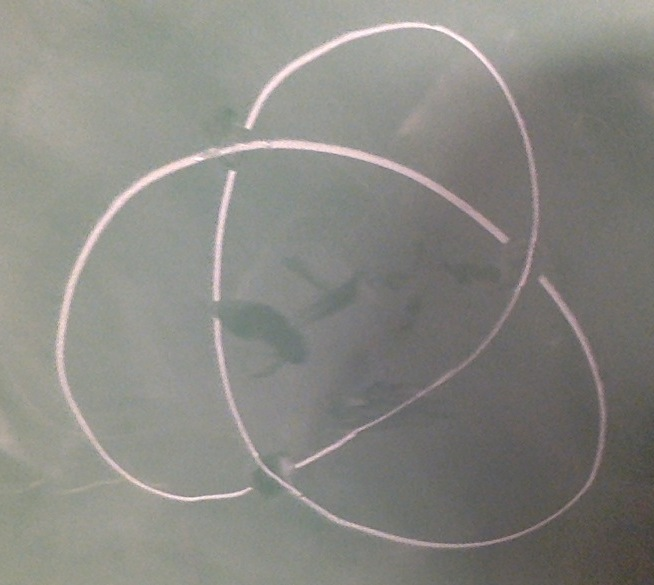
\includegraphics[scale=0.15]{images/trefoil.jpg}

  What is $\fund(\R^3\minus K)$?  Draw two sets of open intervals,
  $A'$ in red and $B'$ in blue, as shown.

  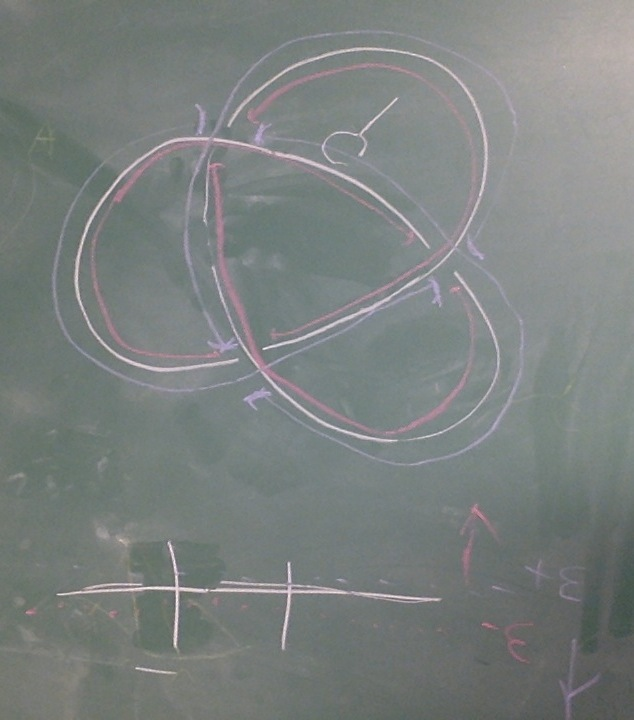
\includegraphics[scale=0.2]{images/trefoil-with-red-and-blue.jpg}

  What looks like the ``ends'' of the ``line segments'' in $A'$, for
  example, are in fact the height of the lines going down to negative
  infinity or up to infinity.  Or you can think of them as ``open
  intervals'', the point being that if there is a little loop (shown
  in white) around one of these, you cannot pull it off the interval,
  since the interval goes on ``forever''.

  $A'$ = $K \cap \{(x,y,z) \in \R^3 \mid z > -\epsilon\}$ ($K$ minus
  the tunnels).

  $B'$ = $K \cap \{(x,y,z) \in \R^3 \mid z < \epsilon\}$ ($K$ minus
  the bridges).

  $A'$ is $m$ open line segments.  In our example, using $K =$
  trefoil, $m = 3$.

  Let $A = (A')^C$.  Then $\fund(A) \isom F_m$, the free group on a
  set of size $m$.

  Let $B = (B')^C$.  Then $\fund(B) \isom F_m$.

  So $A \cap B = \R^3 \minus (A' \union B')$.
  $\fund(A \cap B) \isom F_{2m}$

  ((do we invoke Van Kampbell's theorem here?))

  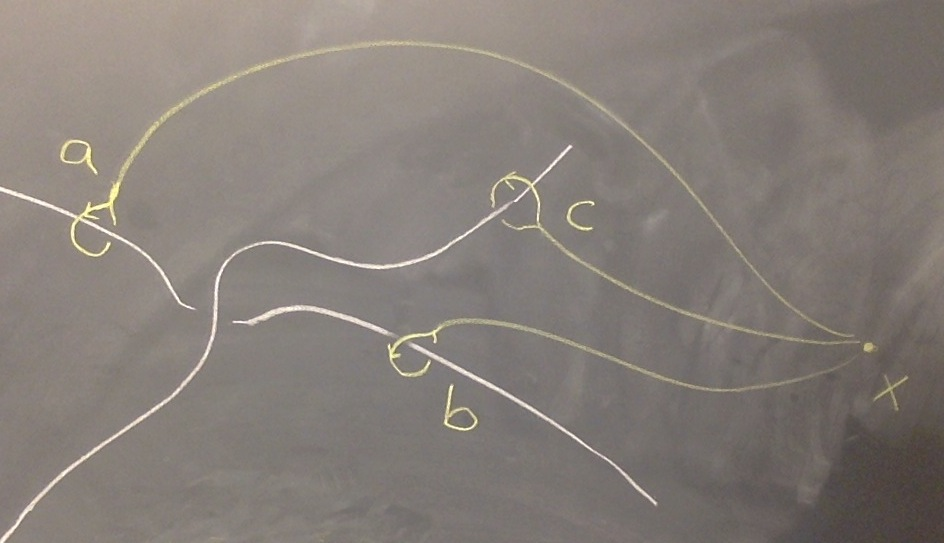
\includegraphics[scale=0.2]{images/mountains.jpg}

  By sliding $a$ under the bridge, we see that $a$ and $b$ are
  conjugate via $c$!

  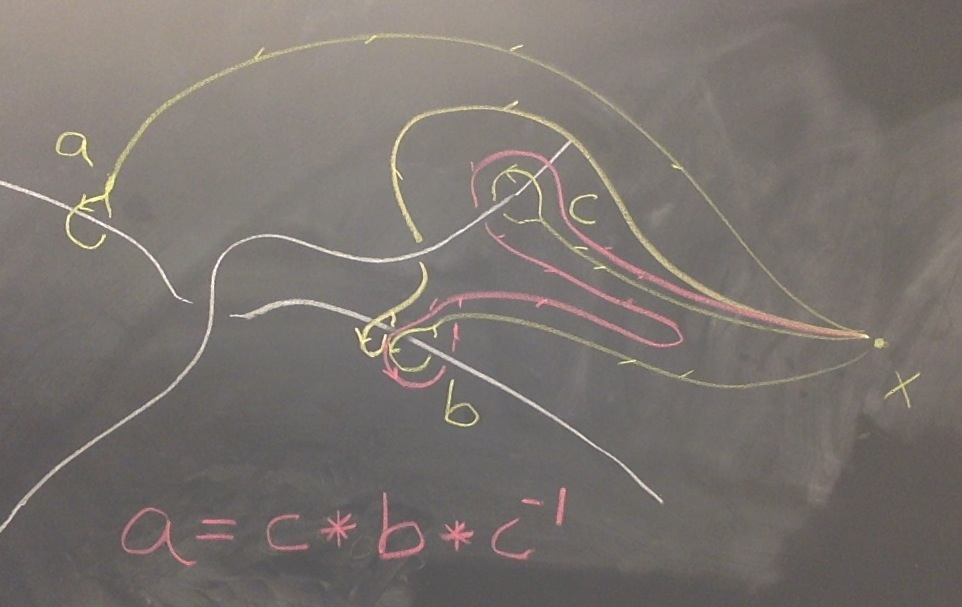
\includegraphics[scale=0.2]{images/mountains-with-explanation.jpg}

  Finally, to compute the fundamental group of $K^C$, we pick an
  arbitrary basepoint $x$ and put loops around the knot as follows.

  We take exactly one loop per open line interval in $A'$.  For each
  crossing, we examine the three loops involved (which are called $a$,
  $b$, and $c$ above) and determine the appropriate conjugate
  relation.  The fundamental group is the group generated by the loops
  and modded out by the relations.

  In the case of the trefoil, the fundamental group
  is $${F_m}/{(a=c*b*c^{-1}, b=a*c*a^{-1}, c=b*a*b^{-1})}$$, as
  illustrated below.

  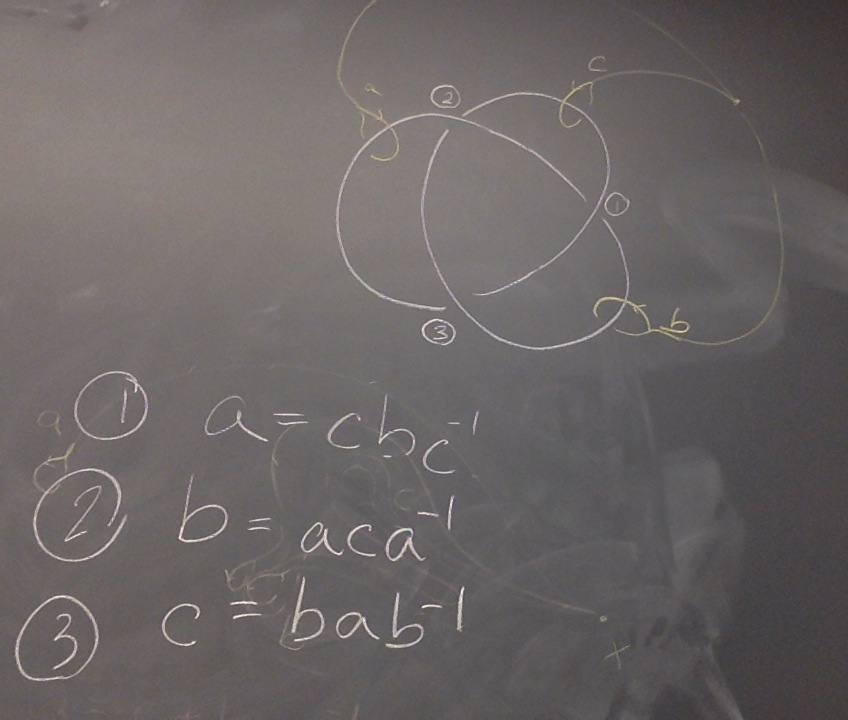
\includegraphics[scale=0.2]{images/trefoil-fully-described.jpg}
\end{example}
\begin{thm}[Wirtinger]
  For any knot $K$, $\fund(\R^3\minus K)$ is generated by loops
  $\gamma_1,,,\gamma_m$ over crossings modulo $a = cbc^{-1}$.
\end{thm}


\section{CW complexes}

CW complexes are like a space built by gluing together balls.
\begin{defn}
  A \de{CW complex} is a space $X$ which is a union of
  $X_0 \subset X_1 \subset \subset \subset$ such that $X_n$ is
  constructed from $X_{n-1}$ by taking
  $X_{n-1} \dunion_{\alpha} D_{\alpha}^n$ modulo identifying (( --> he
  might have meant $S^n$ here.  i think the point is that he meant
  $\d D^n$)) $\phi_\alpha \colon S_\alpha^{n-1} \to X_{n-1}$.  $X_n$
  is called $n$-Skeleton.  $X ~ \phi_\alpha$.

  with topology s.t. $A$ is open iff $A \cap X_n$ is open for all $n$.
\end{defn}
\begin{example}
  $S^n = D^{n-1}/\text{boundary}$ all goes to one point.  $X_0 =$
  discrete set of points.  The $0$-skeleton is a point.  $X_1 =$
  graph. (by connecting the points in $X_0$.)  $X_2 =$ take each cycle
  (can go around multiple times) in $X_1$ and glue it to the boundary
  of a disk (can go around multiple times).
\end{example}
\begin{example}
  ((this example is incomplete and will be repeated next lecture))
  $\R P^n =$ lines in $\R^{n+1}$.

  $\R P^n = \{ \R \dot (1, a_1,,, a_{n-1})\} \isom \R^{n}$.
  $\bunion \{ \R \dot (0, a_1,,, a_{n-1})\} \isom \R P^{n-1}$.
\end{example}

\mydate{d7}{6}{2}{2017}

We wish to show how \(\R P^n\) is a \(CW\)-complex. First let the
\(n-1\) skeleton be \(\R P^{n-1}\). We add the \(n\) cell \(D^n\) to
structure under the gluing map \(S^{n} \to \R P^{n-1}\) where
antipodal points are identified. By induction this gives us a
\(CW\)-complex structure.

\begin{example}[Something that does not admit a \(CW\) structure]
  The topological space known as the \emph{Hawaiian earring} is
  constructed as follows for each \(n \in \Z\) consider the circle of
  radius \(1/n\) tangent to the \(y\)-axis. All of these circles
  together with the subspace topology yield a topological space, call
  it \(X\).

  The only hope for putting a \(CW\) structure on this pace would be
  to consider one \(0\)-cell along with a countable amount of
  \(1\)-cells. However recall that the \(CW\)-structure gain their
  topology through the quotient topology, that is, \(\mathcal{O}\) is
  open in \(X\) if and only if \(q^{-1}(X)\) is open, where \(q\) is
  the glueing map. However any open set centered at the origin
  contains an infinite amount of balls, and thus no such
  \(CW\)-structure may be imposed.
\end{example}

Next we show how to compute \(\pi_1\) of a few
\(CW\)-structures. Using Morse Theory one may show that any compact
manifold admits a \(CW\)-structure.

To compute \(\pi_1\) of the torus one can first decompose it as a
\(CW\)-complex as follows
\begin{align*}
  X_0 &= *\\
  X_1 &= S^1 \vee S^1\\
  X_2 &= D_2
\end{align*}

Then we have that \(\pi_1(T^2) = \pi_1(X_1)/\pi_1(A \cap B)\) where
\(A\) is the boundary of the a square and \(B\) is a smaller square
inside of it. \(A\) is clearly contractible.

When talking about moding out by the fundamental group we are really
talking about moding out by the normal subgroup it generates. In
particular this means that conjugation is trivial, and thus we are
free to pick any basepoint we want. This results in
\[\pi_1(T^2) = \left\langle x,y \mid y^{-1}x^{-1}y x = 1 \right\rangle = \Z
    \times \Z\]

\begin{defn}
  The \emph{connected sum} of two topological spaces \(X\) and \(Y\)
  denoted \(X \# Y \) is given by cutting out some neighborhood of
  each \(X\) and \(Y\) and identifying the new boundary.
\end{defn}


It is easy to see that \(T^2 \# T^2\) is the two holed torus, and in general \(\#^n T^2\) is the \(n\) holed torus.

\end{document}

%%% Local Variables:
%%% mode: latex
%%% TeX-master: "algebraic-topology.tex"
%%% End:
